\section{Scaling law validation}
\label{sec:validation}

\begin{figure}[t]
    \centering
    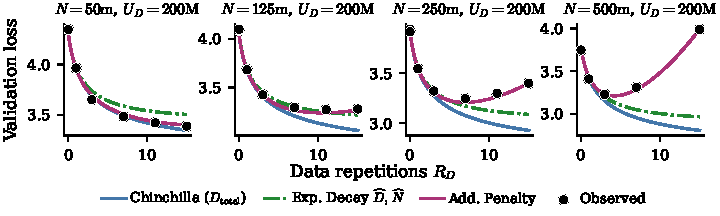
\includegraphics[width=\textwidth]{figures/our_law_fit.pdf}
    \caption{\textbf{Our additive overfitting law adapts to model size.} Predicted vs.\ observed validation loss under different scaling laws. }
    \label{fig:our_law_fit}
    \vspace{-1em}
\end{figure}

\begin{figure}[t]
    \centering

    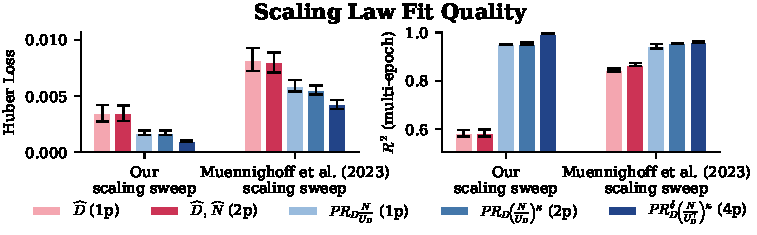
\includegraphics[width=\textwidth]{figures/quantitative_r2_mad.pdf}
    \caption{\textbf{Scaling law fit quality.} Huber loss (left, lower is better) and $R^2$ (right, higher is better) for each scaling law formulation, evaluated on both our scaling sweep and the \citet{muennighoff2023scaling} data. }
    \label{fig:quantitative_r2}
    \vspace{-1em}
\end{figure}

We validate the additive penalty laws (\autoref{eq:one_param}--\autoref{eq:four_param}) against the Chinchilla baseline and the \citet{muennighoff2023scaling} effective-data formulations on two independent scaling sweeps. The first is our own CLM sweep described in \autoref{sec:setup}. The second is the public scaling sweep from \citet{muennighoff2023scaling}, including all runs up to 64 epochs—a more lenient filter than the outlier-removal criteria applied in their original analysis.

\autoref{fig:our_law_fit} compares predicted and observed loss across model sizes. Our proposed law accurately tracks the observed loss across all configurations, capturing the degradation under heavy repetition that the effective-data formulations miss. ~\autoref{fig:quantitative_r2} confirms the quantitative improvement: even our one-parameter additive penalty (\autoref{eq:one_param}) substantially outperforms both the $\widehat{D}(U_D, R_D)$ and $\widehat{D}(U_D, R_D), \widehat{N}(U_N, R_N)$ forms, and the four-parameter form (\autoref{eq:four_param}) achieves near-perfect fit on our data. The improvement extends to the heldout \citet{muennighoff2023scaling} data, where model sizes and repetition ranges span a wider range.

\para{Compute-optimal allocation under repetition.} The superlinear repetition penalty yields qualitatively different compute-optimal allocation advice than prior scaling laws (\autoref{fig:allocation_frontier}). The Chinchilla law, which ignores overfitting, always recommends more repetition: the optimal total token count $D$ grows linearly with compute at fixed $U_D$. The \citet{muennighoff2023scaling} $\widehat{D}(U_D, R_D),\widehat{N}(U_N, R_N)$ form moderates this, prescribing diminishing returns from repetition but never recommending that repetition stop. Our four-parameter law, by contrast, predicts a compute budget beyond which additional repetition is counterproductive. The allocation frontier \emph{turns back}: at high compute, the law recommends scaling model size while \emph{reducing} the number of epochs\footnote{On its surface, this recommendation appears to contradict \citet{muennighoff2023scaling}, who find that data-constrained compute should be allocated toward smaller models trained for more epochs. We trace this disagreement to a methodological choice in their analysis; see \autoref{app:muennighoff_reanalysis}.}, reflecting the overfitting cost of continued repetition. This provides concrete guidance for practitioners: given a fixed data budget, there is a compute level beyond which training a larger model for fewer epochs outperforms training a smaller model for more.

\begin{figure}[t]
    \centering
    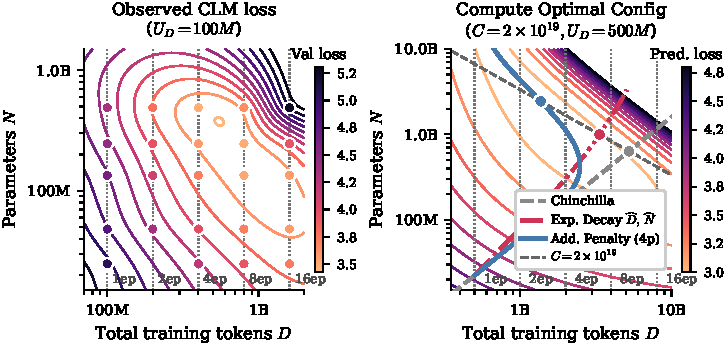
\includegraphics[width=\textwidth]{figures/empirical_vs_model_allocation_100M.pdf}%
    \caption{\textbf{Compute-optimal allocation frontiers.} \textbf{(Left)}~Observed validation loss across our experimental grid ($U_D = 100$M), with contour lines showing the interpolated loss landscape. \textbf{(Right)}~Compute-optimal allocation at $C = 2 \times 10^{19}$ FLOPs and $U_D = 500$M, comparing the Chinchilla law, \citet{muennighoff2023scaling} $\widehat{D}, \widehat{N}$, and our law (\autoref{eq:four_param}).}
    \label{fig:allocation_frontier}
    \vspace{-1em}
\end{figure}

\para{Prescriptive validation.} The $R^2$ comparisons above measure descriptive fit---how well each law explains configurations it was trained on. A more stringent test is \emph{prescriptive} accuracy: given a fixed unique-data and compute budget, does the law recommend the configuration that actually achieves the lowest loss? For each (token budget, compute budget) pair in \autoref{tab:held_out_validation}, we solve each law for the optimal model size and epoch count, train the recommended configuration, and evaluate. Our law consistently recommends larger models with fewer epochs and achieves the best perplexity and downstream performance across all settings.

\begin{table}[t]
    \centering
    \caption{\textbf{Prescriptive validation.} For each (token budget, compute budget) pair, we train the configuration recommended by each scaling law: Chinchilla \citep{hoffmann2022training}, Eff.\ Param.\ \citep{muennighoff2023scaling}, and Ours (\autoref{eq:four_param}). OLMES BPB is the average bits-per-byte across 19 downstream tasks in the OLMES evaluation harness \citep{gu2025olmes}.}
    \label{tab:held_out_validation}
    \begin{tabular}{llllrrr}
        \toprule
        $U_D$ & $C$ & Scaling law & Params & Epochs & Perplexity $\downarrow$ & OLMES BPB $\downarrow$ \\
        \midrule
        \multirow{3}{*}{250M}
        & \multirow{3}{*}{$5 \times 10^{18}$}
        & Chinchilla & 280M & 12 & 25.31 & 1.52 \\
        & & Eff.\ Param.\ & 500M & 7 & 23.91 & 1.50 \\
        & & Ours & 700M & 5 & {22.90} & {1.45} \\
        \midrule
        \multirow{6}{*}{500M}
        & \multirow{3}{*}{$1 \times 10^{19}$}
        & Chinchilla & 390M & 8 & 18.95 & 1.35 \\
        & & Eff.\ Param.\ & 550M & 6 & 18.65 & 1.35 \\
        & & Ours & 700M & 5 & {18.48} & {1.30} \\
        \cmidrule(l){2-7}
        & \multirow{3}{*}{$2 \times 10^{19}$}
        & Chinchilla & 670M & 10 & 18.90 & 1.37 \\
        & & Eff.\ Param.\ & 950M & 7 & 19.34 & 1.40 \\
        & & Ours & 2.2B & 3 & {17.73} & {1.34} \\
        \bottomrule
    \end{tabular}
    \vspace{-1em}
\end{table}

\para{Generalization to external data.} To test the generalizability of our scaling law form, we apply it to the published data from \citet{muennighoff2023scaling}, which was completely held out during the development of our scaling law. It therefore represents a true test of generalization. They make different choices with respect to backbone architecture (GPT-2 versus Llama-2), tokenization, etc. for pre-training. We find that the additive penalty forms significantly  outperforms the \citet{muennighoff2023scaling} formulations on their own published data, confirming that the improvement generalizes across pre-training implementations.
